%---------------------------------------------------------------------
\subsubsection{Minuta de reunião (28-maio-2015)}

\begin{tabbing}
  Local \= xxx \kill
  Local \> : LEAD \\
  Data  \> : 28 de Maio de 2015 \\
  Hora  \> : 10:00
\end{tabbing}

%---------------------------------------------------------------------
\participantes{
  \elael,
  \gabriel,
  \julia,
  \patrick,
  \alana,
  \ramon,
  \renan.
}

\textbf{Aprovação da minuta}

\textbf{Update semanal do Projeto EMMA}
  
\textbf{\renan.} 
	\begin{itemize}
		\item \textbf{Tarefas concluídas:}
			\begin{itemize}    
				\item Ajustes de conceito da escotilha inferior.
			\end{itemize}
		
		\item \textbf{Novas tarefas:}
			\begin{itemize} 
				\item Formalizar ajustes no EMMA SOTA
			\end{itemize}
	\end{itemize}
	
\textbf{\elael.} 
    \begin{itemize}    
		\item \textbf{Tarefas concluídas:}
			\begin{itemize}
				\item Análise de torc e vibração.
				\item Explorou possibilidades para menosr vibração.
				\item Possibilidades relacionadas ao tamanho de braço do robô
			\end{itemize}
			
		\item \textbf{Novas tarefas:}
			\begin{itemize} 
				\item ver com Ramon se será necessário o uso de um 'demper'ou não.
				\item Ver a menos velocidade na qual a base permitirá a continuidade do
				processo de coating.
				\item Frmalizar alterações no SOTA.
			\end{itemize}
	\end{itemize}
	
\textbf{\gabriel.} 
	\begin{itemize}
		\item \textbf{Tarefas concluídas:}
			\begin{itemize}    
				\item Problemas relacionados ao ambiente da unidade geradora.
				\item Ë preciso entender como a curvatura do ambiente pode alterar a
				estabilidade do braço.
			\end{itemize}
		\item \textbf{Novas tarefas:}
			\begin{itemize}
				\item Parafusos nmmagnéticos: qual teria de ser o peso para segurar a base.
				Efeitos colaterais de agua, pressão e deformidade do ambiente.
				\item Frmalizar alterações no SOTA.		
			\end{itemize}
	\end{itemize}
	
\textbf{\julia.} 
	\begin{itemize}
		\item \textbf{Tarefas concluídas:}
			\begin{itemize}    
				\item Relatório Administrativo concluído.
				\item Entrevistas com orientadores de Mestrado. 
			\end{itemize}
		\item \textbf{Novas tarefas:}
			\begin{itemize}
				\item Apresentação EMMA, formalizar  projeto para divulgação.
				\item Roteiro para vídeo EMMA Aevo.
			\end{itemize}
	\end{itemize}
%   \item Problemas em aberto:
%   \begin{itemize}
%     \item Procedimento de compras e medidas para as instalações finais do
%     laboratório.
%     \item Opções para a comprar de software, Adobe/ Solid Works/ Live
%     Meeting/Bibliografia
%     \item Fechar orçamento Inventário.
%     \item Criar log para documentar problemas de ROCK/ criar um forum para
%     colaboração (?!)
%     \item Dropbox para compartilhamento de arquivos.
%     \item Viagem ESB/Relatório:
%   \end{itemize}

\textbf{Agenda para a próxima reunião:}
	\begin{itemize}
		\item Resultado de pesquisas individuais.
	    \item Viagem Jirau Abril.
	    \item Novas tarefas \& recomendações.
	\end{itemize}


\vspace{5mm}%
\parbox[t]{70mm}{
  Aprovado por: \\[5mm]
  \centering
  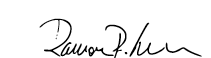
\includegraphics[width=65mm]{figs/logo/assinatura-ramon.png} \\[-4mm]
  \rule[2mm]{70mm}{0.1mm} \\
  \ramon \\[1mm]
  Coordenador do Projeto \\
}

%---------------------------------------------------------------------
\fim


